\section{Deployment Diagram}
In order to obtain a photo of the splint a camera is used, then that image is being passed to the program that performs the recognition process.
\begin{figure}[h]
	\centering
	
\includegraphics[width=\textwidth]{images/deployment_diagram}
	\caption{Deployment Diagram}
\end{figure}

\section{Image Acquisition}
\paragraph{}
Images used while developing the program were shot on a regular iPhone. Also the light conditions were far from ideal. Plenty of images contain either light reflexes or extensive shades. Moreover, image background and surroundings differ which makes the processing more error prone.

\begin{figure}
	\centering
	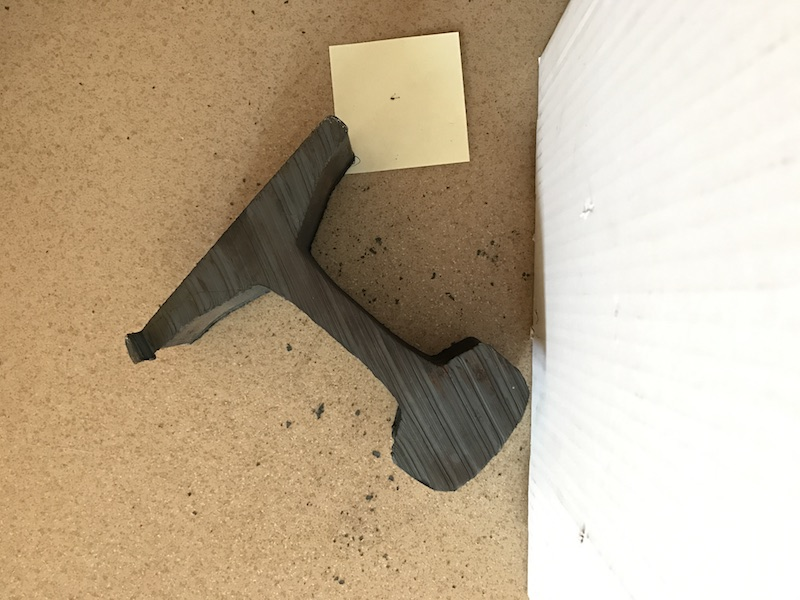
\includegraphics[width=\textwidth]{images/example_splint}
	\caption{Example image of a splint}
\end{figure}

% Write about first attempts to tackle it with artificially prepared images
 
\paragraph{}
However, provided the system will be implemented in production use, professional equipment will be installed (for example high quality camera) and maximal effort will be undertaken to ensure similar light conditions and background (ideally striking, monochromatic colour)

\section{Image Preprocessing}
\paragraph{}
Before computing the "barcode" representation of the splint there is a couple of steps required to enable processing. The primary goal is to extract the shape of the split from the image, effectively ignoring everything else. Let us now look at the first attempt to approach this task using following techniques:

\begin{enumerate}
	\item Image thresholding (binary) - it is a function that for a given grayscale pixel assigns one of two values {A, B}. A is assigned to all of the pixels with value greater than some threshold value and B otherwise.
	$$
	threshold (pixel, T) = \begin{cases}
		A, pixel.value > T \\
		B, pixel.value <= T
	\end{cases}
	$$
	\item Finding contours - a function finding curves joining continuous points, having same colour or intensity
\end{enumerate}

\begin{algorithm}{\textbf{Extracting the shape of the split - first approach}}
	\begin{algorithmic}[1]
		\Function{extract}{$grayscale$}
			\State $threshold \gets \textbf{cv2.threshold}(grayscale)$
			\State $contours \gets \textbf{cv2.findContours}(threshold)$
			\State $splintContour \gets \textbf{maxArea}(contours)$
			\State $mask \gets \textbf{createMask}(splintContour)$
			\State \textbf{return} $\textbf{cropImage}(grayscale, mask)$
		\EndFunction
	\end{algorithmic}	
\end{algorithm}

The pseudocode presented above greatly simplifies the usage of OpenCV library. It does not provide any of the other required parameters for library functions and it also discards other return values. Function steps provide just the essential parts of the algorithm to present the idea. Regarding abstract functions, please ignore implementation details and just note that:
\begin{enumerate}
	\item \textbf{maxArea()} - finds the contour with maximal area amongst ones provided as the parameter
	\item \textbf{createMask()} - creates a mask that includes the whole shape of contour (i.e. the edge and the interior) for a given contour
	\item \textbf{cropImage()} - to a given image applies a given mask, effectively cutting out just those pixels specified by the mask 
\end{enumerate}

\paragraph{}
Further development of the preprocessing algorithm led to a little bit more complex series of steps. Instead of converting whole RGB image to grayscale, the multi-channel array is split into separate single-channel arrays. Empirical experiments showed that for the given set of input images best results can be obtained when using just the red color channel. The thresholding phase is now executed with threshold value computed from the histogram (first, peak value that corresponds to the splint is found and then after performing simple algebraic operations is used to obtain the value). The thresholding process returns a binary image where white color denotes area that is most likely a part of the splint and a black color otherwise. Such a binary image then undergoes a series of corresponding image blurring (using median blur filter) and morphological opening (which is a series of erosions followed by dilations). To complete the process and fill some gaps that may have appeared in some of the previous phases, a fill holes procedure is applied.

\begin{algorithm}{\textbf{Extracting the shape of the split - improved approach}}
	\begin{algorithmic}[1]
		\Function{extract}{$image$}
			\State $redChannel \gets$ R channel from the $image$
			\State $splintPeak \gets$ Splint peak from histogram of $redChannel$
			\State $threshold \gets \textbf{threshold}(redChannel, splintPeak)$
			\State $blur \gets \textbf{cv2.medianBlur}(threshold)$
			\For{$i \gets 0\ \textbf{to}\ repetitions$}
				\State $opening \gets \textbf{open}(blur)$
				\State $blur \gets \textbf{cv2.medianBlur}(opening)$
			\EndFor
			\State $filled \gets \textbf{fillHoles}(blur)$
			\State $contours \gets \textbf{cv2.findContours}(filled)$
			\State $splintContour \gets \textbf{maxArea}(contours)$
			\State $mask \gets \textbf{createMask}(splintContour)$
			\State \textbf{return} $\textbf{cropImage}(grayscale, mask)$
		\EndFunction
	\end{algorithmic}	
\end{algorithm}

\begin{figure}[H]
     \centering
     \subfloat[Before]{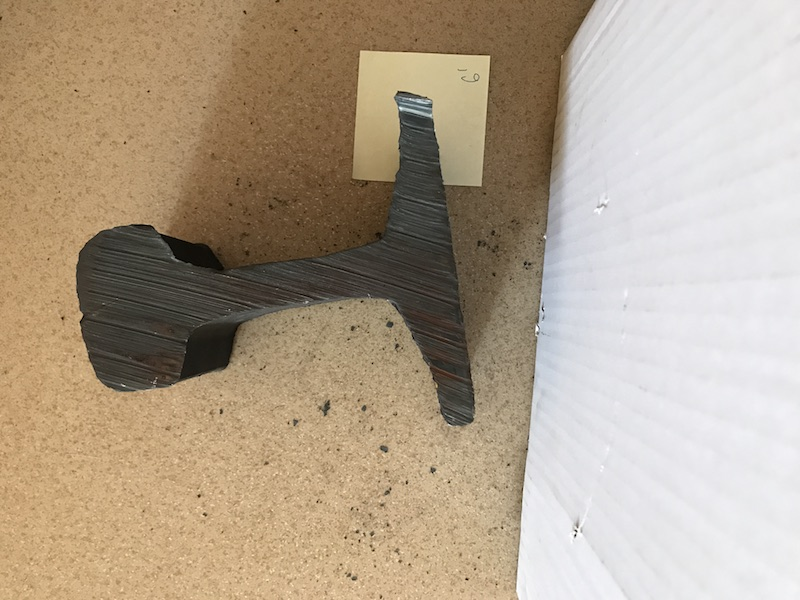
\includegraphics[width=0.45\textwidth]{images/good_before_preprocessing}}
     \qquad
     \subfloat[After thresholding]{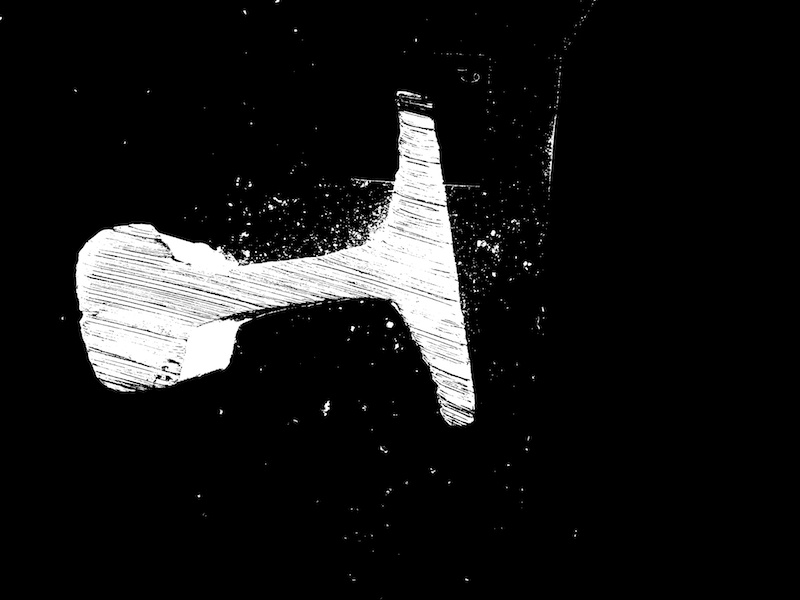
\includegraphics[width=0.45\textwidth]{images/good_after_thresholding}}
     \qquad
     \vfill
     \subfloat[After opening and blurring]{
\includegraphics[width=0.45\textwidth]{images/good_after_opening_and_blurring}}
     \qquad
     \subfloat[Shape detected]{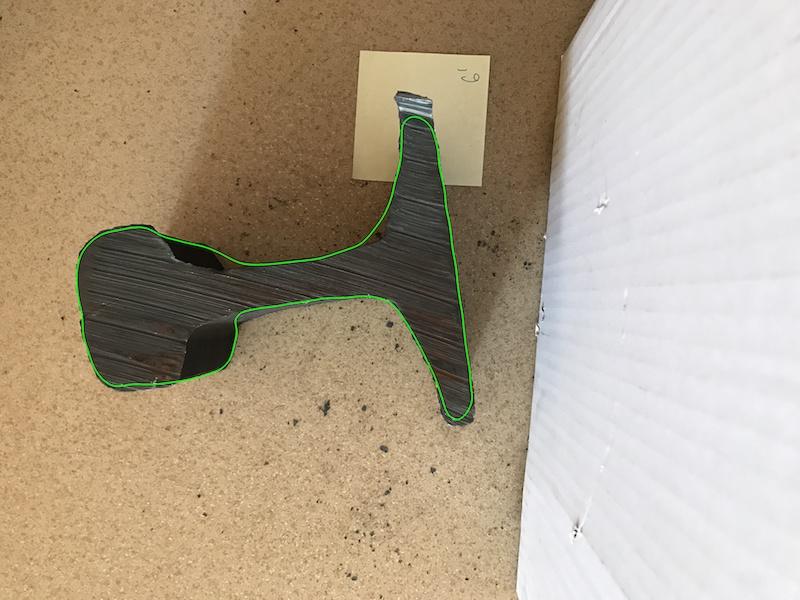
\includegraphics[width=0.45\textwidth]{images/good_after_preprocessing}}
     \caption{Stages of preprocessing - successful}
\end{figure}

\begin{figure}[H]
     \centering
     \subfloat[Before]{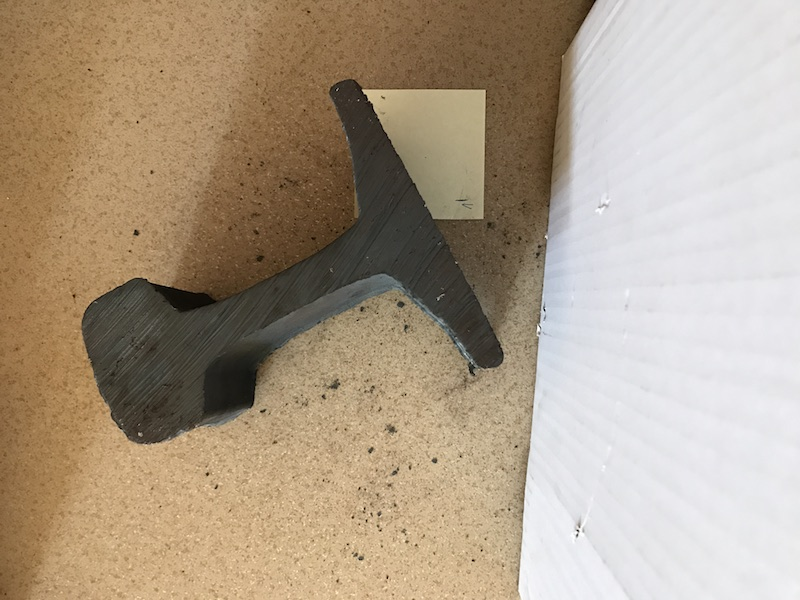
\includegraphics[width=0.45\textwidth]{images/medium_before_preprocessing}}
     \qquad
     \subfloat[After thresholding]{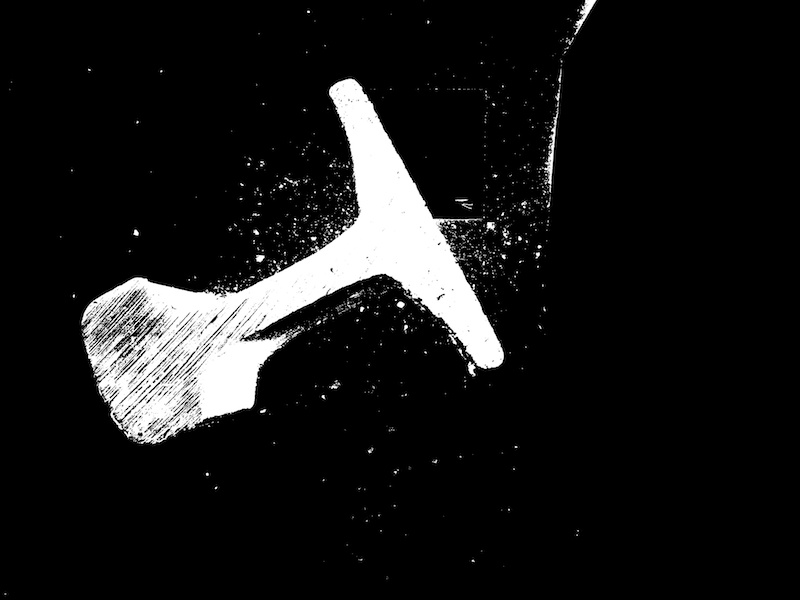
\includegraphics[width=0.45\textwidth]{images/medium_after_thresholding}}
     \qquad
     \vfill
     \subfloat[After opening and blurring]{
\includegraphics[width=0.45\textwidth]{images/medium_after_opening_and_blurring}}
     \qquad
     \subfloat[Shape detected]{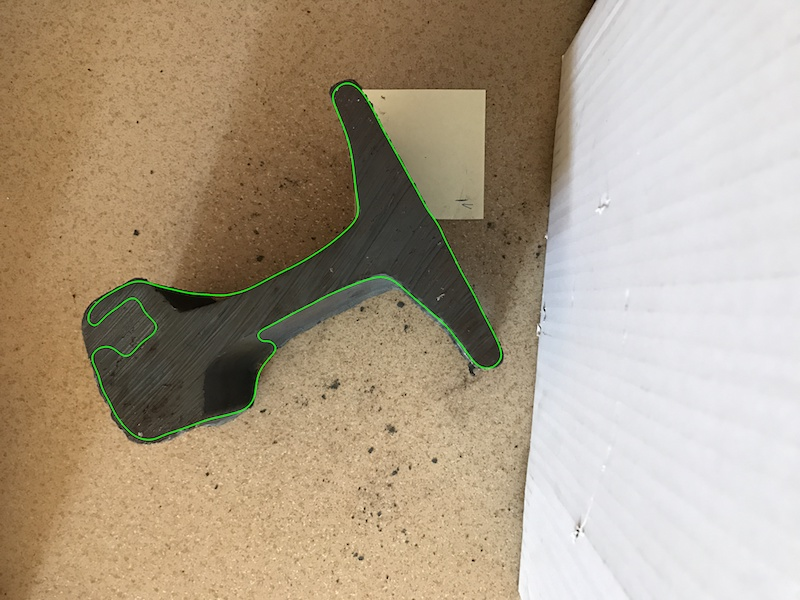
\includegraphics[width=0.45\textwidth]{images/medium_after_preprocessing}}
     \caption{Stages of preprocessing - still good}
\end{figure}

\section{Image Processing}
\paragraph{}
Finally, at the stage of image processing, the input in an image containing only (hopefully) the shape of the splint. 